\documentclass{ctexart}

\usepackage{amsmath}

\usepackage{amsthm}

\usepackage{amssymb}

\usepackage{bm}

\usepackage{graphicx}

\usepackage{listings}
\lstset{
basicstyle=\scriptsize
}

\usepackage{caption}

\begin{titlepage}

\title{微分方程数值解 \\ 第四周作业}

\author{于慧倩 \\ 14300180118}

\date{2017年3月}

\end{titlepage}

\begin{document}

\maketitle

\newpage

\begin{enumerate}
%第一题

\item 证明隐式Euler格式是一阶收敛的。

\begin{proof}
对于测试方程\( \frac{\mathrm{d} u}{\mathrm{d} t}=au\),说明隐式Euler格式是收敛的。

要说明Euler格式是收敛,需要说明在\(Delta t\)趋于零时,在固定的\(T=N \Delta t\)时刻,\(e_N=u(T)-u_N\)也趋于零。对于\(e_n=u(t_n)-u-n\),可以得到

\[ e_n =u_0e^{at_n} - u_0 \frac{1}{(1-a \Delta t)^n}=u_0 e^{at_n}(1-e^{-n\ln(1-a \Delta t)-at_n})\]

Taylor展开后,另有\(t_n=n\Delta t\)

\begin{eqnarray*}
e^{-n\ln(1-a \Delta t)-at_n} &=& 1-n \ln(1-a\Delta t) - at_n+ \frac{1}{2} [n \ln(1-a \Delta t)+at_n]^2+\dots  \nonumber \\
&=&1-n(-a\Delta t-\frac{1}{2}a^2\Delta t^2)-at_n+\frac{1}{2}n^2a^2\Delta t^2+\frac{1}{2}a^2t_n^2-a^2t_nn\Delta t +O(\Delta t^3) \nonumber \\
&=&1+\frac{1}{2}a^2t_n\Delta t +O(\Delta t^3) \nonumber \\
\end{eqnarray*}
最终有
\[e_n=u_0e^{at_n}(-\frac{a^2t_n}{2}\Delta t+O(\Delta t^2)) \]
从这个表达式可以看出,对于固定的\(T=N \Delta t\),在\(T\)时刻的误差\( | u(T)-u_N | \leq C\Delta t\),相对误差\( \frac{| u(T)-u_N | }{|u(t_n)|} \leq \frac{a^2t_n}{2}\Delta t+O(\Delta t^2) \).为一阶收敛。
\end{proof}


\item 用显式、隐式、改进的、修正的Euler格式计算\(\frac{\mathrm{d}u}{\mathrm{d}t}=au,u_0=1,a=2,T=1\),并用图说明收敛性。

分别取步长\(t=0.02,t=0.1\)依次做出显式、隐式、改进的、修正的Euler格式如下:
\newpage
\[t=0.02\]

\centerline{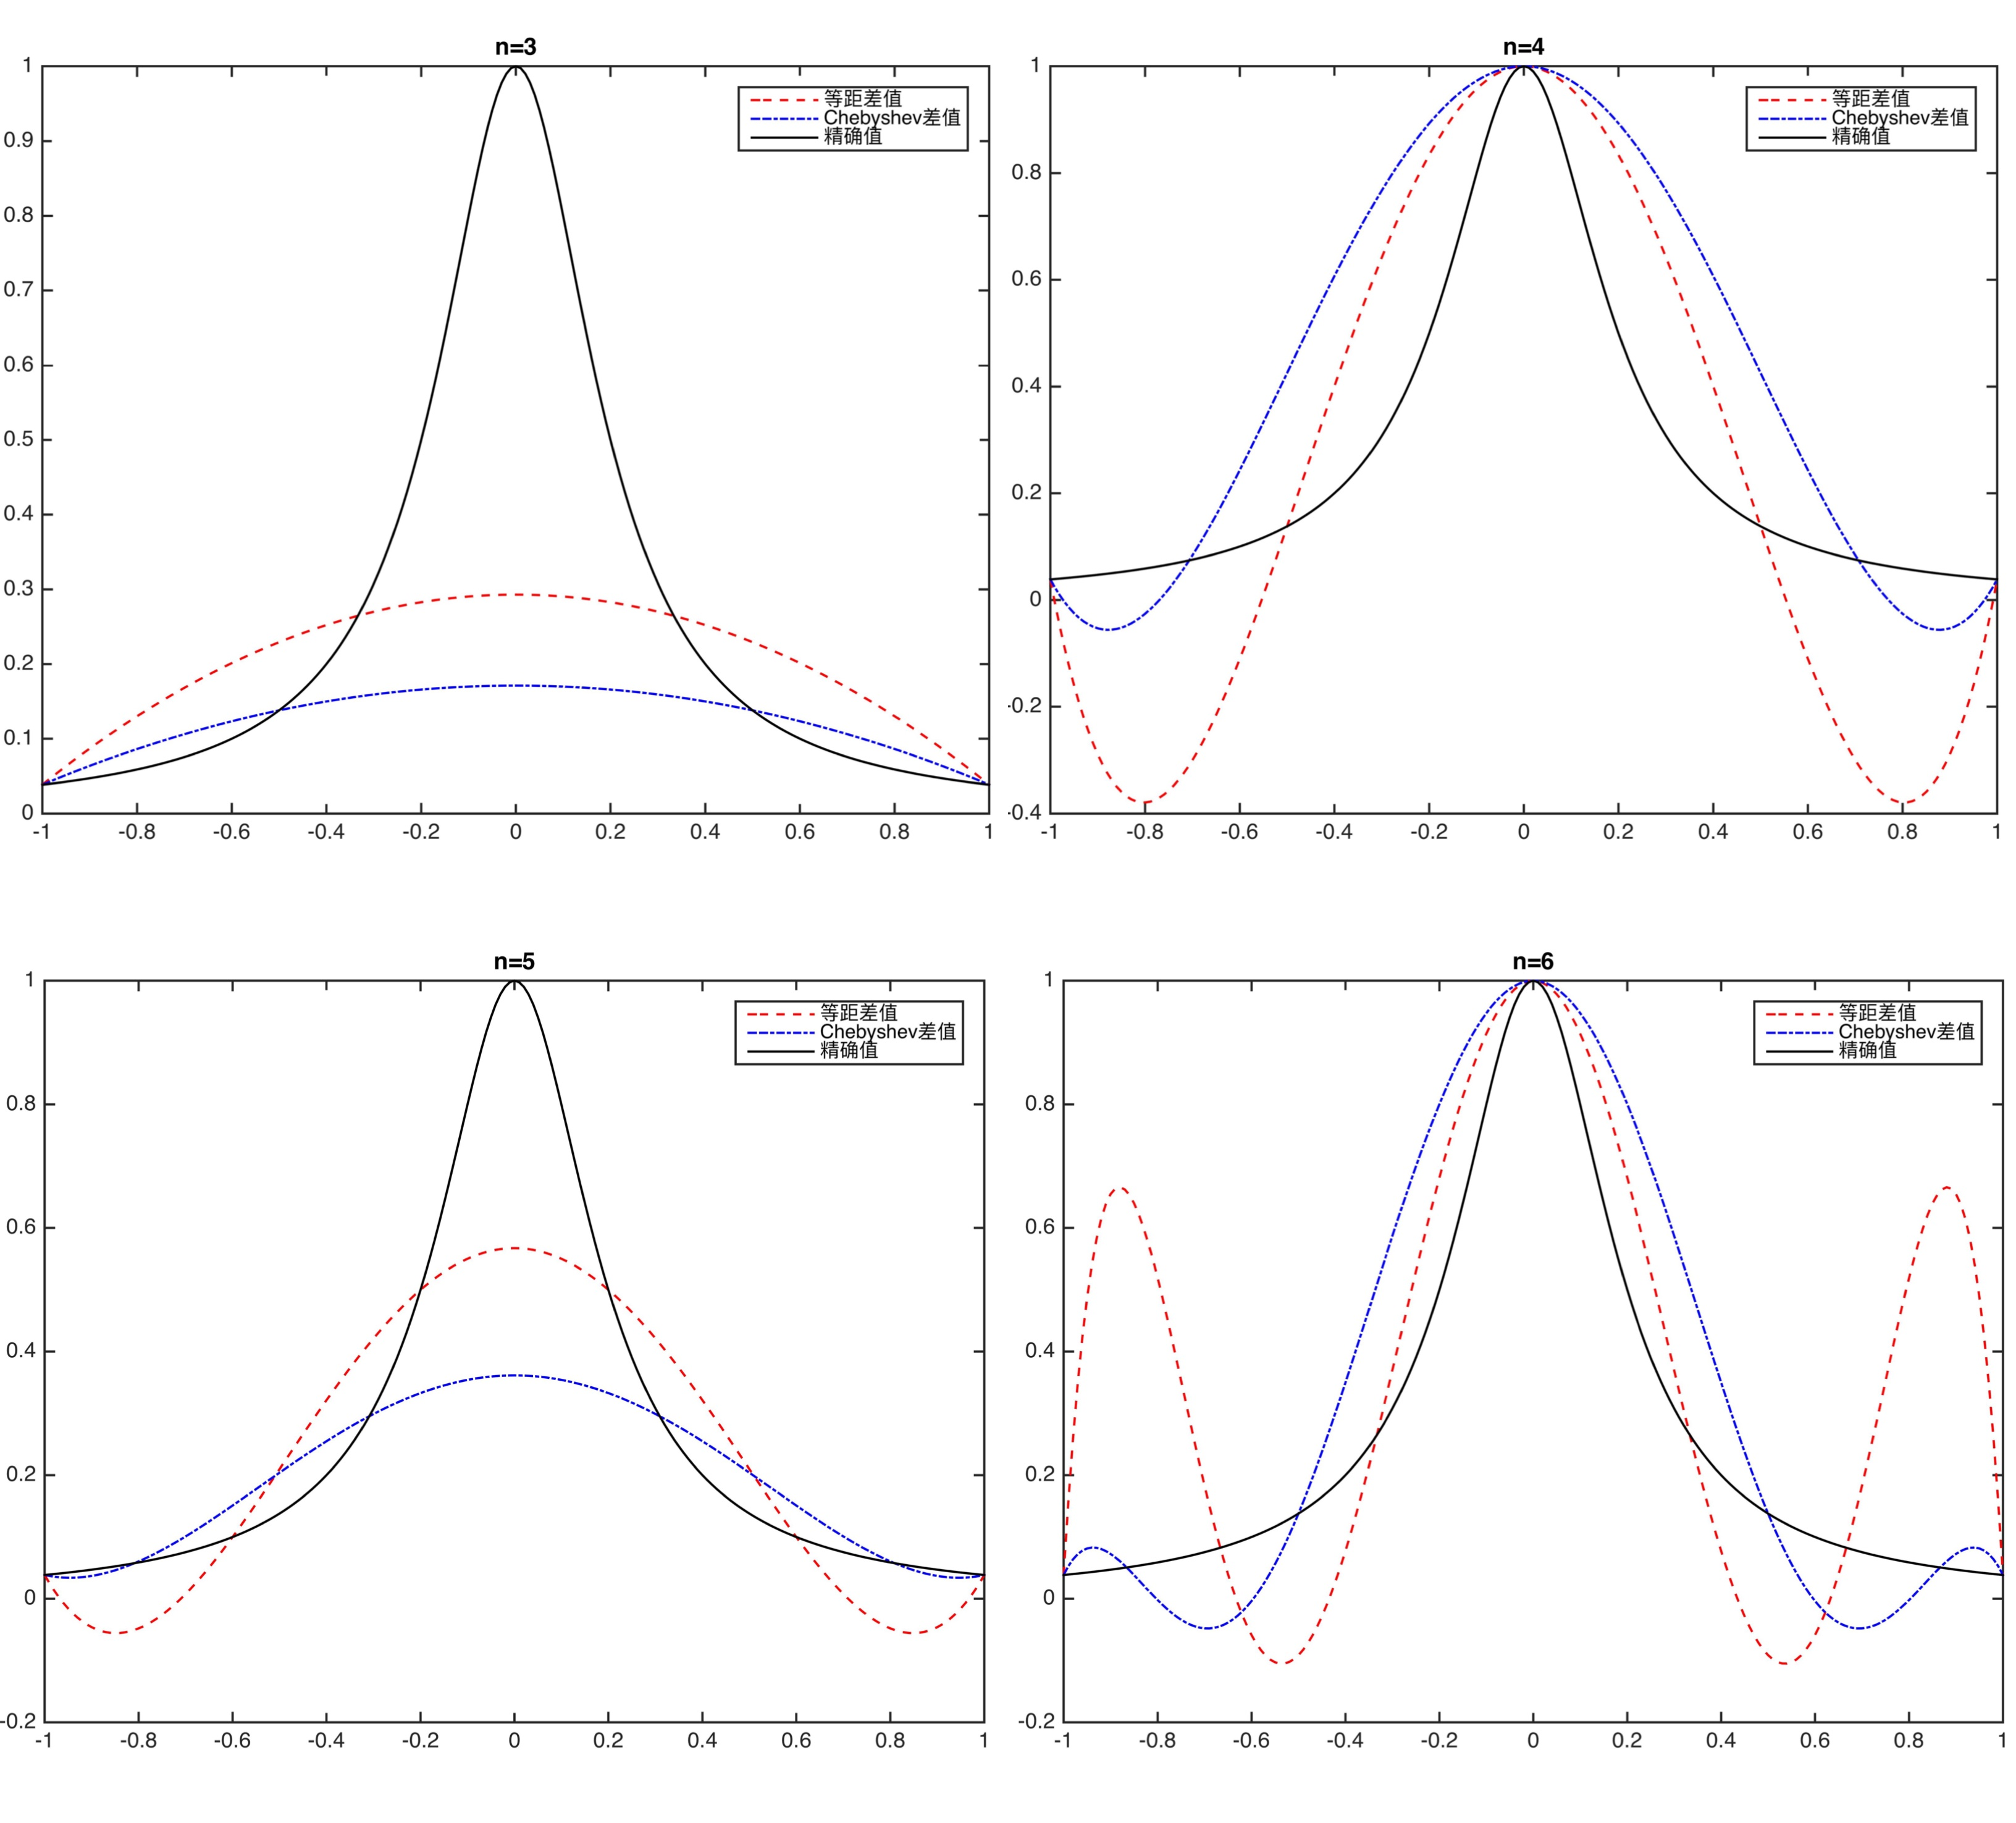
\includegraphics[width=3.5in]{1.jpg}}

\[t=0.1\]

\centerline{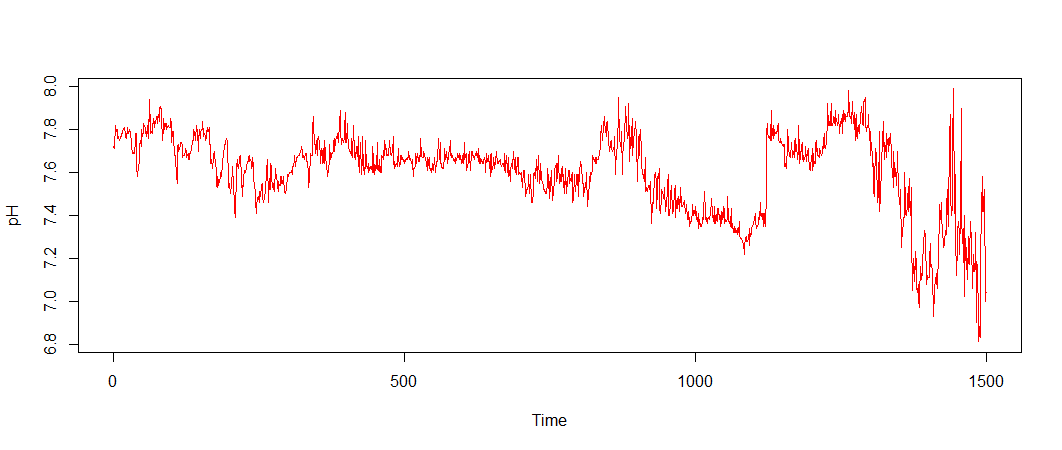
\includegraphics[width=3.5in]{2.jpg}}

从图中可以清楚地看出当步长较小或步长较大时,改进的和修正的Euler格式收敛速度都很快,且都明显快于显式、隐式的Euler格式收敛状况,显式Euler格式比真值偏小,隐式Euler格式比真值偏大。


\end{enumerate}

\end{document}
